\documentclass[xcolor=dvipsnames,handout,t]{beamer}
% use handout in document class to stop transitions

\mode<presentation>
{
  \usetheme{Madrid}%{Madrid}
  % or ..AnnArbor, Boadilla, CambridgeUS, Copenhagen, default, Frankfurt, Goettingen, Hannover
  %       Montpellier, PaloAlto, Rochester, Szeged,

  \setbeamercovered{invisible}
  % or whatever (possibly just delete it)
}
\usepackage{color,empheq}
\usepackage{subfigure}
\usepackage{caption}
\usepackage{subcaption}
\usepackage[english]{babel}
\usepackage{xmpmulti,animate}
\usecolortheme{seahorse} %this makes the colors less strong.

\usepackage{times}
% Or whatever. Note that the encoding and the font should match. If T1
% does not look nice, try deleting the line with the fontenc.
\usepackage{graphicx}
%\usepackage{tcolorbox}
\usepackage{tikz,lipsum,lmodern}
\usepackage[most]{tcolorbox}
\usepackage{amsfonts,amssymb,amsmath,mathtools}
      % use Times fonts if available on your TeX system
\usepackage{epsfig}
\usepackage{hyperref}
\usepackage{changepage}
\usepackage[utf8]{inputenc}
\usepackage[T1]{fontenc}
%\usepackage{animate,movie15,media9}
%\usepackage{multimedia}

\newcommand{\todo}[1]{\textcolor{orange}{\texttt{TODO: #1}}} 
\newcommand{\red}[1]{\textcolor{red}{#1}} 
\newcommand{\bl}[1]{\textcolor{blue}{#1}} 


\usetikzlibrary{shapes}

\title[] % (optional, use only with long paper titles)


%\subtitle
%{Presentation Subtitle} % (optional)

\title[Forecasting GRBs w/ GWs] % (optional, use only with long paper titles)
{Forecasting Gamma-ray Bursts with Gravitational Waves}

\subtitle{\todo{Add background image}} % (optional)

\author[Sarp Akcay]{Sarp Akcay\inst{1}\inst{2} }
\institute[FSU Jena - UCD] % (optional, but mostly needed)
{
  \inst{1}%
  FSU Jena %and University College Dublin
  \inst{2}%
  University College Dublin
  }


%\vspace{-3cm}
%\titlegraphic{
%  \vspace{1.75cm}  \includegraphics[width=1.0cm]{figs/ucd.png}%\hspace*{1cm}~\includegraphics[height=1cm]{figs/missing_inch.jpg} \hspace*{1cm}  \includegraphics[width=1.0cm]{figs/ucd.png}
%}
\date[Sabanci University]{14 November 2018}

\subject{Talks}

\usefonttheme[onlymath]{serif}
\setbeamerfont{frametitle}{size=\huge}
\setbeamercolor{frametitle}{fg=Black,bg=White}

\newcommand{\Mag}{\textcolor{magenta}}
\newcommand{\Red}{\textcolor{red}}
\newcommand{\Blue}{\textcolor{blue}}
\renewcommand{\c}{\cos}
\renewcommand{\t}{\theta}
\renewcommand{\b}{\bar}
\newcommand{\f}{\frac}
\newcommand{\bt}{\beta}
%\newcommand{\s}{\sin}
\newcommand{\ph}{\phi}
\newcommand{\g}{\gamma}
\newcommand{\nn}{\nonumber}
\newcommand{\la}{\lambda}
\newcommand{\al}{\alpha}
\newcommand{\La}{\Lambda}
\newcommand{\el}{\ell}
\newcommand{\h}{\hat}
\newcommand{\mrm}{\mathrm}
\newcommand{\ord}{\mathcal{O}}
\newcommand{\F}{\mathcal{F}}
\newcommand{\be}{\begin{equation}}
\newcommand{\ee}{\end{equation}}
\newcommand{\ba}{\begin{eqnarray}}
\newcommand{\ea}{\end{eqnarray}}
\newcommand{\bi}{\begin{itemize}}
\newcommand{\ei}{\end{itemize}}
\newcommand{\bef}{\begin{frame}}
\newcommand{\ef}{\end{frame}}
%\newcommand{\h}{\bar{h}}
\newcommand{\bs}{\begin{small}}
\newcommand{\es}{\end{small}}
\newcommand{\parallelsum}{\mathbin{\!/\mkern-5mu/\!}}
\newcommand{\Lim}[1]{\raisebox{0.5ex}{\scalebox{0.8}{$\displaystyle \lim_{#1}\;$}}}
\newcommand*\circled[1]{\tikz[baseline=(char.base)]{\node[shape=circle,draw,inner sep=2pt] (char) {#1};}}
%------------------ for coloured boxes in math modes --------------------
% Syntax: \colorboxed[<color model>]{<color specification>}{<math formula>}
\newcommand*{\colorboxed}{}
\def\colorboxed#1#{%
  \colorboxedAux{#1}%
}
\newcommand*{\colorboxedAux}[3]{%
  % #1: optional argument for color model
  % #2: color specification
  % #3: formula
  \begingroup
    \colorlet{cb@saved}{.}%
    \color#1{#2}%
    \boxed{%
      \color{cb@saved}%
      #3%
    }%
  \endgroup
}
%%-------------------------------------------------------------------------

% tikz boxes
\newcommand\TBox[3][]{%
  \tikz\node[draw,ultra thick,red,text width=#2,align=left,#1] {#3};}

\setbeamertemplate{frametitle}[default][center]



\begin{document}
%{
%\usebackgroundtemplate{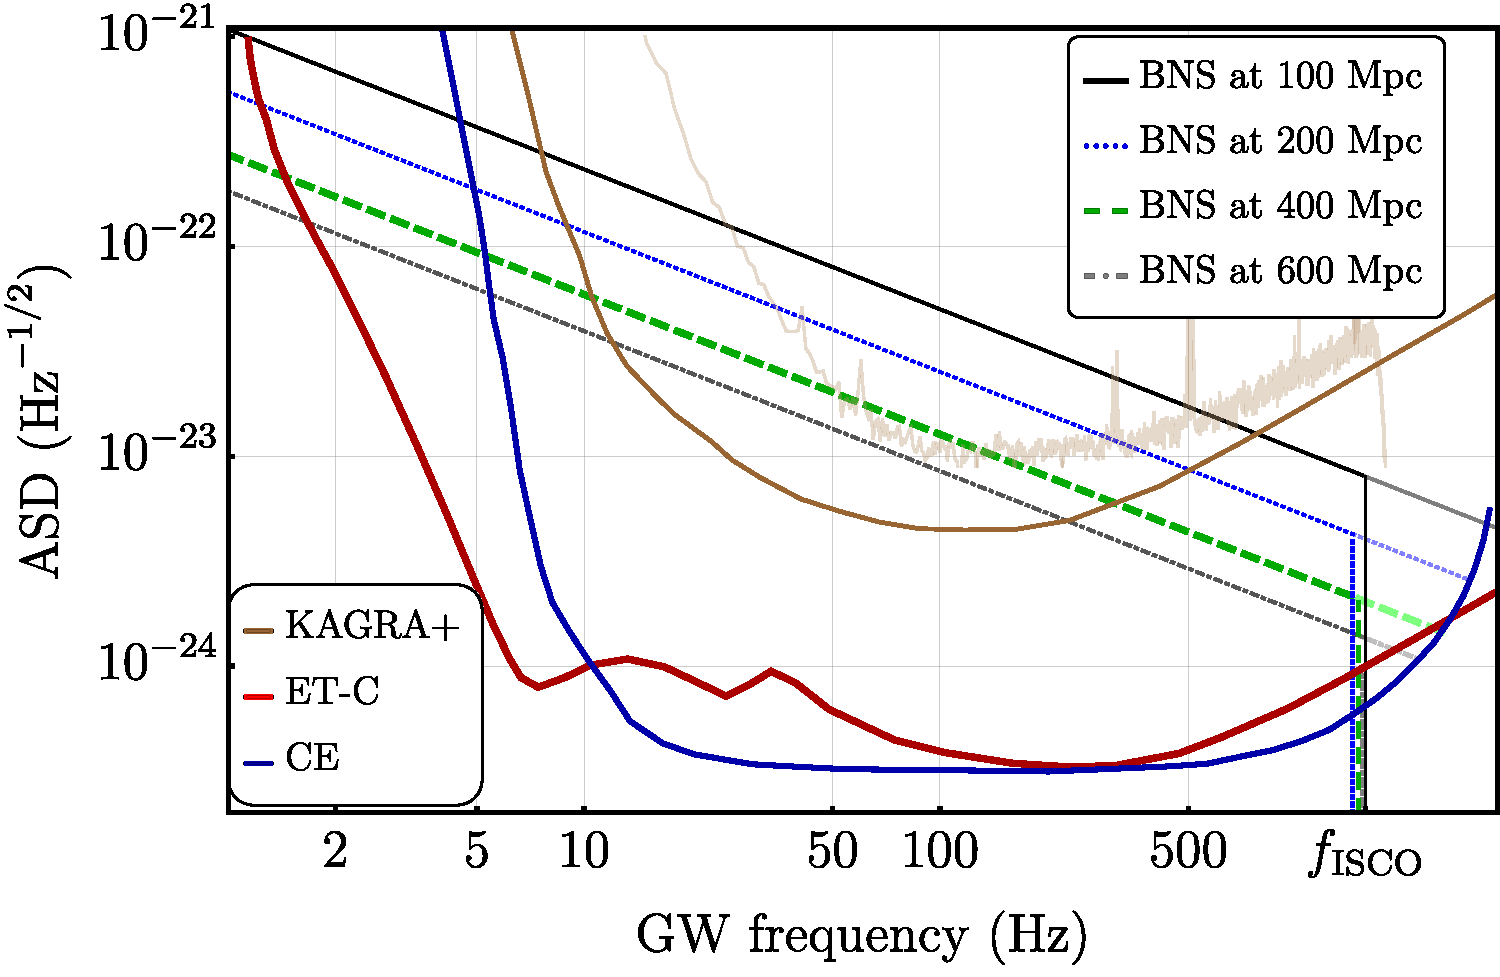
\includegraphics[width=1\paperwidth,height=\paperheight]{../Figures/ET_strains_redshifted_v2.pdf}}
\begin{frame}
 \titlepage
\end{frame}
%}

\begin{frame}{Outline}
\begin{itemize}
 \item Motivation
 \item Gravitational waves
 \item Binary neutron star inspirals
 \item Gravitational-wave detectors
 \item Event rates 
\end{itemize}
\todo{finish this slide remove later if short on time}

 
\end{frame}


\begin{frame}{Motivation: Multi-messenger Astronomy}
\begin{itemize}
 \item \emph{Multi}: two fundamentally different waves from common events.
 \item[]\quad Gravitational waves (GWs): ``hearing''  the universe.
 \item[]\quad Electromagnetic waves (EWs): ``seeing'' the universe.
 \item \red{GW170817}-\bl{GRB170817A}-\textcolor{brown}{AT2017gfo}: the ``event'' \\
 \quad inspiral + merger of two neutron stars (GWs) \\
 \ \ = short-hard gamma-ray burst + kilonova (EWs)
 \item[] Broad-band in gravitational waves: 10Hz - 2000Hz
 \item[] Ultra broad-band in electromagnetic waves: gamma rays to radio.
 \item A simple question \\
{\small ``What can we offer to the astronomy community with future GW detections?''}
 \end{itemize}


 \end{frame}

 
\begin{frame}{Gravitational waves: Einstein 1916}
  \begin{center}
\begin{tikzpicture}
            \node[anchor=south west,inner sep=0] at (0,0) {\includegraphics[height=3.5cm]{figs/Einstein1916.png}};
            %\draw<1>[red,ultra thick,rounded corners] (1.6,1) rectangle (\textheight-1cm,5);
           \uncover<3->{\draw<3->[red,thick] (1.7,0.04) rectangle (3.1,0.27);}
        \end{tikzpicture}
        \\
         \uncover<2->{Perturbations of spacetime with speed $=c$, sourced by accelerating masses.}
         \end{center}
          \begin{itemize}
 \item  \uncover<3->{Spacetime metric $g_{\mu\nu} = \eta_{\mu\nu} + h_{\mu\nu}$, \quad with $| h_{\mu\nu} | \ll 1$.}
 \item  \uncover<4->{Insert into $G_{\mu\nu} = 0$. Keep only $\mathcal{O}(h)$. Pick a gauge.} %(e.g. Lorenz).}
  \uncover<5->{\[ \Rightarrow\quad \Box \bar{h}_{\mu\nu}= 0, \quad \text{wave equation!} \]}
  \item \uncover<6->{\alert{Plane-waves:} $ \bar{h}_{\mu\nu} = \Re\left[A_{\mu\nu}\, \text{e}^{i k_\mu x^\mu}\right] =\Re\left[A_{\mu\nu}\, \text{e}^{-i\omega (t-z/c )}\right]$.}
 \end{itemize}
\end{frame}

\begin{frame}{Gravitational waves: d.o.f.'s}
$A_{\mu\nu} $ is the polarization tensor.
\begin{itemize}
 \uncover<2->{\item $\{ \bar{h}_{\mu\nu}, A_{\mu\nu} \}$: $4\times4$, symmetric \uncover<3->{$\hspace{1.5cm}\Rightarrow \f{4\times 5}{2}\ \ \ = 10$ d.o.f.}}
 \uncover<4->{\item Gauge condition: $\nabla_\mu \bar{h}^{\mu\nu} =  A_{\mu\nu} k^\nu= 0$ \uncover<5->{$\Rightarrow10-4 = \, 6$ d.o.f.}}
 \uncover<6->{\item Residual gauge freedom \hspace{2.25cm} \uncover<7->{$\Rightarrow 6-4 \ \ = \alert{2}$ \alert{d.o.f.}}}
 %\uncover<7->{\vspace{2mm}\begin{center}$ \bar{h}'_{\mu\nu} = \bar{h}_{\mu\nu} - \xi_{\mu,\nu} - \xi_{\nu,\mu} + \eta_{\mu\nu} \nabla_\alpha \xi^\alpha . $ \end{center}\vspace{2mm}}
\end{itemize}
\uncover<7->{\quad \ Consistent with $\pm 2$ helicities of a \bl{massless} spin 2 boson.\\}
\uncover<8->{$\Rightarrow$ \alert{2} POLARIZATIONS (\alert{transverse}): \uncover<10->{$\begin{array}{l}A_{xx}=-A_{yy} = \red{h_+}  \\ A_{xy}=\ \ A_{yx} = \red{h_\times}  \\ \end{array}$}}
\\
\todo{Replace with Maggiore's discussion?}
{\begin{center} \includegraphics[height=2.79875cm]{figs/white_box.png}\end{center}}
\end{frame}
 
 

\begin{frame}{Gravitational waves: d.o.f.'s}
%\begin{center}
%\animategraphics[loop,controls,width=3cm]{12}{GWs_frame-}{0}{29} 
%\end{center}
$A_{\mu\nu} $ is the polarization tensor.
\begin{itemize}
{\item $\{ \bar{h}_{\mu\nu}, A_{\mu\nu} \}$: $4\times4$, symmetric {$\hspace{1.5cm}\Rightarrow \f{4\times 5}{2}\ \ \ = 10$ d.o.f.}}
 {\item Gauge condition: $\nabla_\mu \bar{h}^{\mu\nu} =  A_{\mu\nu} k^\nu= 0${ $\Rightarrow10-4 = \,6$ d.o.f.}}
 {\item Residual gauge freedom \hspace{2.25cm}{ $\Rightarrow 6-4 \ \ = \alert{2}$ \alert{d.o.f.}}}
 %{\vspace{2mm}\begin{center}$ \bar{h}'_{\mu\nu} = \bar{h}_{\mu\nu} - \xi_{\mu,\nu} - \xi_{\nu,\mu} + \eta_{\mu\nu} \nabla_\alpha \xi^\alpha . $ \end{center}\vspace{2mm}}
\end{itemize}
{\quad \ Consistent with $\pm 2$ helicities of a \bl{massless} spin 2 boson.\\}
{$\Rightarrow$ \alert{2} POLARIZATIONS (\alert{transverse}): {$\begin{array}{l}A_{xx}=-A_{yy} = \red{h_+}  \\ A_{xy}=\ \ A_{yx} = \red{h_\times}  \\ \end{array}$}}
\\
\todo{Replace with Maggiore's discussion?}
{\begin{center} \animategraphics[loop,controls,height=2.4cm]{12}{GWs_plus-}{0}{20} \hspace{1cm} \animategraphics[loop,controls,height=2.4cm]{12}{GWs_cross-}{0}{20}\end{center}}
\end{frame}

\begin{frame}{Making gravitational waves}{non-spherical, accelerated motion}
 \alert{Inspirals}, GRBs, bumps on neutron stars, supernovae, the Big Bang. \\% (BICEP 2).\\
 \uncover<2->{Gravitational-wave luminosity: \uncover<3->{\alert{quadrupole} radiation}  (leading-order)}
 \uncover<3->{\begin{center} $ \boxed{\dot{E}=L_\text{GW} = \f{G}{c^5} \langle (\partial_t^3 \bar{Q}_{ij})^2 \rangle}$\\\vspace{2mm}}
 \uncover<4->{\begin{small}$ \quad \bar{Q}_{ij} = Q_{ij}-\frac{1}{3}\delta_{ij}Q^k_k, \quad Q^{ij} = \int \rho(t,{\mathbf x})x^i x^j d^3 x $ \end{small} \end{center}}
 \uncover<5->{{\bf Binary systems:} 2 points masses in circular orbit. }
 
\end{frame}

\begin{frame}{Making gravitational waves}{non-spherical, accelerated motion}
 \alert{Inspirals}, GRBs, bumps on neutron stars, supernovae, the Big Bang. \\%  (BICEP 2).\\
 Gravitational-wave luminosity: \alert{quadrupole} radiation (leading-order)
 \begin{center} $ \boxed{\dot{E}=L_\text{GW} = \f{G}{c^5} \langle (\partial_t^3 \bar{Q}_{ij})^2 \rangle}$\\ \vspace{2mm}
 \begin{small}$ \quad \bar{Q}_{ij} = Q_{ij}-\frac{1}{3}\delta_{ij}Q^k_k, \quad Q^{ij} = \int \rho(t,{\mathbf x})x^i x^j d^3 x $ \end{small} \end{center}
 {\bf Binary systems:} 2 points masses in circular orbit.\todo{$R\to r$ in vid}
 \begin{tikzpicture}[overlay,remember picture]
\onslide<5->\node (img0 )[anchor=center,scale=1,opacity=1] at ([shift={(-3.8cm,-2.8cm)}]current page.center) {\animategraphics[loop,controls,height=2.4cm]{12}{Circ_Orb-}{0}{20}};
\onslide<2->\node (t1 )[anchor=center,scale=1,opacity=1] at ([shift={(2cm,-1.3cm)}]current page.center) {$\mu=m_1 m_2/M^2,\ x(t) = r \cos\Omega t, \ y(t) = r \sin\Omega t $};
\onslide<3->\node (t2 )[anchor=center,scale=1,opacity=1] at ([shift={(2.25cm,-2.2cm)}]current page.center) {$ Q^{ij} =  2 M\, x^i x^j, \qquad \boxed{\dot{E} = \f{32}{5}\f{G\mu^2}{c^5}r^4 \Omega^6}$};
\onslide<4->\node (t3 )[anchor=center,scale=1,opacity=1] at ([shift={(2.5cm,-3.2cm)}]current page.center) {Enhancement due to \bl{$e$} (Peters \& Mathews).};
\onslide<5->\node (t3 )[anchor=center,scale=1,opacity=1] at ([shift={(2cm,-4cm)}]current page.center) {$ \bl{\f{\left(1 + \f{73}{24}e^2+ \f{37}{96} e^4 \right)}{(1-e^2)^{7/2}}}$};
\end{tikzpicture}
\end{frame}








 \begin{frame}{Binary Neutron Star Inspirals}
 Notation:
 \begin{itemize}
  \item $\red{f} $: GW frequency.
  \item $\omega\equiv2\pi f = 2\Omega$: GW angular frequency.
  \item $t$: observer/detector time \quad$ \Longrightarrow\quad\dot{Y}= dY/dt$.
 \end{itemize}

  Assumptions:
  \begin{itemize}
   \item Quasi-circular orbits: $e \ll 1$ and $\tfrac{|\dot{r}|}{r\Omega} <10^{-3} $ at $f=100\,$Hz.
   \item Point masses: tidal effects for $f \gtrsim 100\,$Hz
   \item Set $m_1 =m_2 = 1.4 M_\odot$, constraints: $1.2 M_\odot \lesssim m_\text{NS}\lesssim 1.6M_\odot$.
   \item Use Newtonian/post-Newtonian theory ($\le$3.5{\bf PN}).
   \item Terminate inspiral at Schwarzschild ISCO \todo{add ISCO curve?}
   \begin{footnotesize}
   \[f_\text{ISCO} = \f{c^3}{6^{3/2}\pi G M} \simeq 1571 \left(\f{2.8M_\odot}{M}\right)\text{Hz}\] 
   \end{footnotesize}
   \item Quadrupolar GWs only: higher modes suppressed by $\tfrac{m_1-m_2}{M}\tfrac{v^2}{c^2}$
   \item Neglect spins: spin-orbit $\tfrac{\dot{E}_\text{SO}}{\dot{E}} \sim \tfrac{v_s}{c}\tfrac{v}{c}\tfrac{R_\text{NS}}{r}$, spin-spin $\sim \tfrac{v^4}{c^4}$
  \end{itemize}

 \end{frame}


\begin{frame}{Binary Neutron Star Inspirals}{Newtonian evolution}
 Define \bl{chirp mass} \hspace{1.cm} $\red{M_c} \equiv \mu^{3/5} M^{2/5} = \tfrac{(m_1 m_2)^{3/5}}{(m_1+m_2)^{1/5}}$ \\
 %and symmetric mass ratio\qquad $\nu \equiv \tfrac{\mu}{M} =\tfrac{m_1 m_2}{M^2}$\\
 \vspace{1mm}
 which gives, using Kepler's \bl{third law}: $\Omega^2 = G M r^{-3}=\omega^2/4$   
 \begin{footnotesize}
  $$ \boxed{\dot{E} = \f{32}{5}\f{c^5}{G} \left(\f{G M_c\, \omega}{2c^3}\right)^{10/3}}$$
 \end{footnotesize}\\
%
{\bf Key idea:} \red{energy balance} between $\dot{E}$ and \\
$\tfrac{d}{dt}$ of gravitational binding energy
$ E_b= -\tfrac{G m_1 m_2}{2r} = -\left(\tfrac{G^2 M_c^5 \omega^2}{32}\right)^{1/3} $
%
\[ 
 \dot{E}(f) = -\dot{E}_b(f) \Longrightarrow \boxed{\red{\dot{f}} = \f{96}{5}\pi^{8/3} \f{(G M_c)}{c^5}^{5/3}\, \red{f^{11/3}} }
 \]
\[
 \red{ \dot{f} \propto f^{11/3}\quad(1)}
\]

\begin{tikzpicture}[overlay,remember picture]
\node[draw, red,thick,minimum width=3cm,minimum height=0.75cm] (b) at (5.9,0.85){};
\end{tikzpicture}

\end{frame}

\begin{frame}{Binary Neutron Star Inspirals}{Inspiral time}
Integrate $\dot{f} \sim f^{11/3} \quad \Longrightarrow \quad \int dt \sim \int f^{-11/3}df \quad\Rightarrow\quad t \sim \red{f^{-8/3}}$
\\
\vspace{1mm}
Fix integration constant $\tau = t_\text{coal} - t >0$. \\
\vspace{2mm}
Introduce \red{inspiral time}, i.e, time to BNS \bl{coal}escence
%
\begin{align}
 \red{\tau_\text{insp}(f)} &= \f{5}{256\pi}\f{c^5}{(\pi G M_c)^{5/3}} \,{f^{-8/3}}\nn\\
 &\simeq \red{16.72\,\text{minutes}} \, \left(\f{1.219 M_\odot}{M_c}\right)^{5/3}\,\red{\left(\f{10\,\text{Hz}}{f}\right)^{8/3}\quad(2)}\nn
\end{align}
Number of GW cycles to coalescence: $\int \tfrac{f}{\dot{f}}df\sim f^{-5/3}$ %$\int df {f}/\dot{f}$
\begin{align}
 \red{\mathcal{N}_\text{cyc}(f)} %&=\f{1}{32\pi} \f{c^5}{(\pi G M_c)^{5/3}}\left[ f^{-5/3}-f_\text{max}^{-5/3}\right]\nn \\
 &\approx 1.605\times \red{10^4 \left(\f{10\,\text{Hz}}{f} \right)^{5/3}}\,\left(\f{1.219 M_\odot}{M_c}\right)^{5/3}\quad \red{(3)}\nn
\end{align}
%
\begin{tikzpicture}[overlay,remember picture]
\node[draw, red,thick,minimum width=8.2cm,minimum height=1.3cm] (b) at (7.,3.35){};
\node[draw, red,thick,minimum width=10cm,minimum height=1.3cm] (b) at (6.2,1){};
\end{tikzpicture}
%
\end{frame}

\begin{frame}{Gravitational waves from BNS}
TT gauge, multipole, slow-velocity expansions give \todo{add suppl. slide}
\[
 h_{ij}^\text{TT} = \tfrac{1}{D}\tfrac{2G}{c^4} \ddot{Q}_{il}^\text{TT}(t-z/c)
\]
%
 \begin{align}
 h_+(t) &= h_c(t)\, \left(\f{1+\cos^2\iota}{2}\right)\, \cos[\Phi(t)],\label{eq:hplus_TD}\\
 h_\times(t) & =h_c(t)\,\cos\iota \sin[\Phi(t)]\label{eq:hcross_TD},
\end{align}
%
%
where
%
\begin{align}
h_c(t) &=\f{4}{D}\left(\f{G M_c}{c^2}\right)^{5/3}\, \left(\f{\pi f(t)}{c}\right)^{2/3} \nn\\
\Phi(t) &=\int_{t_i}^t dt' \omega(t') + \text{PN corrections}
\end{align}


Frequecny increases as $f^{11/3}$\\
Amplitude increases as $f^{2/3} \Longrightarrow$ \red{Chirp!} 

\end{frame}



 \begin{frame}{GW Detectors: Interferometers}
  Geodesic deviation
 \end{frame}










\begin{frame}{Supplement 1: mode suppression}
\begin{itemize}
 \item For $q=1$ due to symmetry only (2,2), (3,2), (4,2), (4,4) are nonzero 
 \item For $q\ne 1$ all $\ell \ge 2$ modes exist, but are much smaller than $(2,2)$
\end{itemize}

 
\end{frame}











\end{document}


